\subsection{Mediciones}
\bigskip
\subsubsection{Polarización}
Al medir la polarización del circuito se regulo el multiplicador Vbe de forma tal de obtener corrientes similares a la salida. En el Cuadro~\ref{polarizacion} se observan las mediciones que se tomaron para verificar la correcta polarización del circuito.


\begin{table}[H]
\begin{center}
\label{polarizacion} 
\begin{tabular}{|c|c|}
\hline 
\textbf{Resistor} & \textbf{Tensión entre bornes} \\ 
\hline 
RL & $59.2\mvolt$ \\ 
\hline 
R17 & $14.2\mvolt$ \\ 
\hline 
R18 & $15.8\mvolt$ \\ 
\hline 
R10 & 137.8mV \\ 
\hline
R5 & 21.3mV \\ 
\hline
R2 & 20.8mV \\ 
\hline
R4 & 4.187V \\ 
\hline
R8 & 659.4mV \\ 
\hline
\end{tabular} 
\end{center}
\end{table}

\medskip
\subsubsection{Ganancia}
Con una entrada senoidal de 1kHz cuya amplitud se fue variando y registrando las tensiones de salidas sobre la carga de $8\ohm$ se realizo el Cuadro~\ref{ganancia}. De estas mediciones se obtiene que la ganancia es de 23 veces$\simeq$ 27.2dB. Por otro lado, la última medición confirma que se cumple el requerimiento de potencia a la salida, ya que se obtienen 65.6W RMS.


\begin{table}[H]
\begin{center}
\label{ganancia} 
\begin{tabular}{|c|c|}
\hline 
\textbf{Vin(pico)} & \textbf{Vout(pico)} \\ 
\hline 
200mV & 4.6V \\ 
\hline 
500mV & 11.5 \\ 
\hline 
1 & 23V \\ 
\hline 
1.41V1 & 32.4V \\ 
\hline
\end{tabular} 
\end{center}
\end{table}

\medskip
\subsubsection{Respuesta en Frecuencia}
Obtencion de banda de frecuencia en que la ganancia se mantiene constante con un error de 0.1dB.
Estas mediciones se realizaron ingresando una señal senoidal, de amplitud tal, que sobre la carga hubiese 2V pico. Luego se buscaron frecuencias donde la ganancia decreciera 0.1dB, esto es, tension pico de 1.97V a la salida.

\begin{itemize}
\item Frecuencia inferior: $7.7\hertz$
\item Frecuencia superior: $85\khertz$
\end{itemize}


\medskip
\subsubsection{Impedancia de Entrada}

Para realizar esta medición se aplico senoidal de 1kHz y de amplitud tal que a la salida del amplificador hubiese una de 6V pico. Luego se agrego en serie con la entrada una resistencia de 4.7$\kohm$ y un potenciómetro de 10$\kohm$, al que se fue variando hasta que la salida mostrara 3V pico. Por lo tanto, la resistencia de entrada del amplificador y la del serie resistor-potenciómetro eran iguales, midiendo esta última se obtuvo una resistencia de entrada de 10.52$\kohm$.
\medskip
\subsubsection{Impedancia de Salida}

Se determino el valor de la impedancia de salida midiendo la tensión de salida dos veces,
una en vacío (Vo) y otra con carga nominal (Vc) y a una frecuencia de 1 KHz. Resultando:


\begin{itemize}
\item Vo = 2,2939 
\item Vc = 2.2750 
\item $R_{carga}$ = 8.4$\ohm$
\end{itemize}

Luego se puede calcular la impedancia de salida (asumiendo que es totalmente resistiva) con la expresión: 
$$
Zo = R_{carga} \times (\frac{Vo}{Vc} -1) \simeq 0.07 \ohm
$$
\medskip
\subsubsection{Slew Rate}

Para obtener elvalor del Slew Rate del circuito se procedió a ingresar una señal rectangular de 1kHz al amplificador y observar la salida del mismo. Los resultados se muestran en la Figura~\ref{slew_rate_completo}.

\begin{figure}[H]
\centering
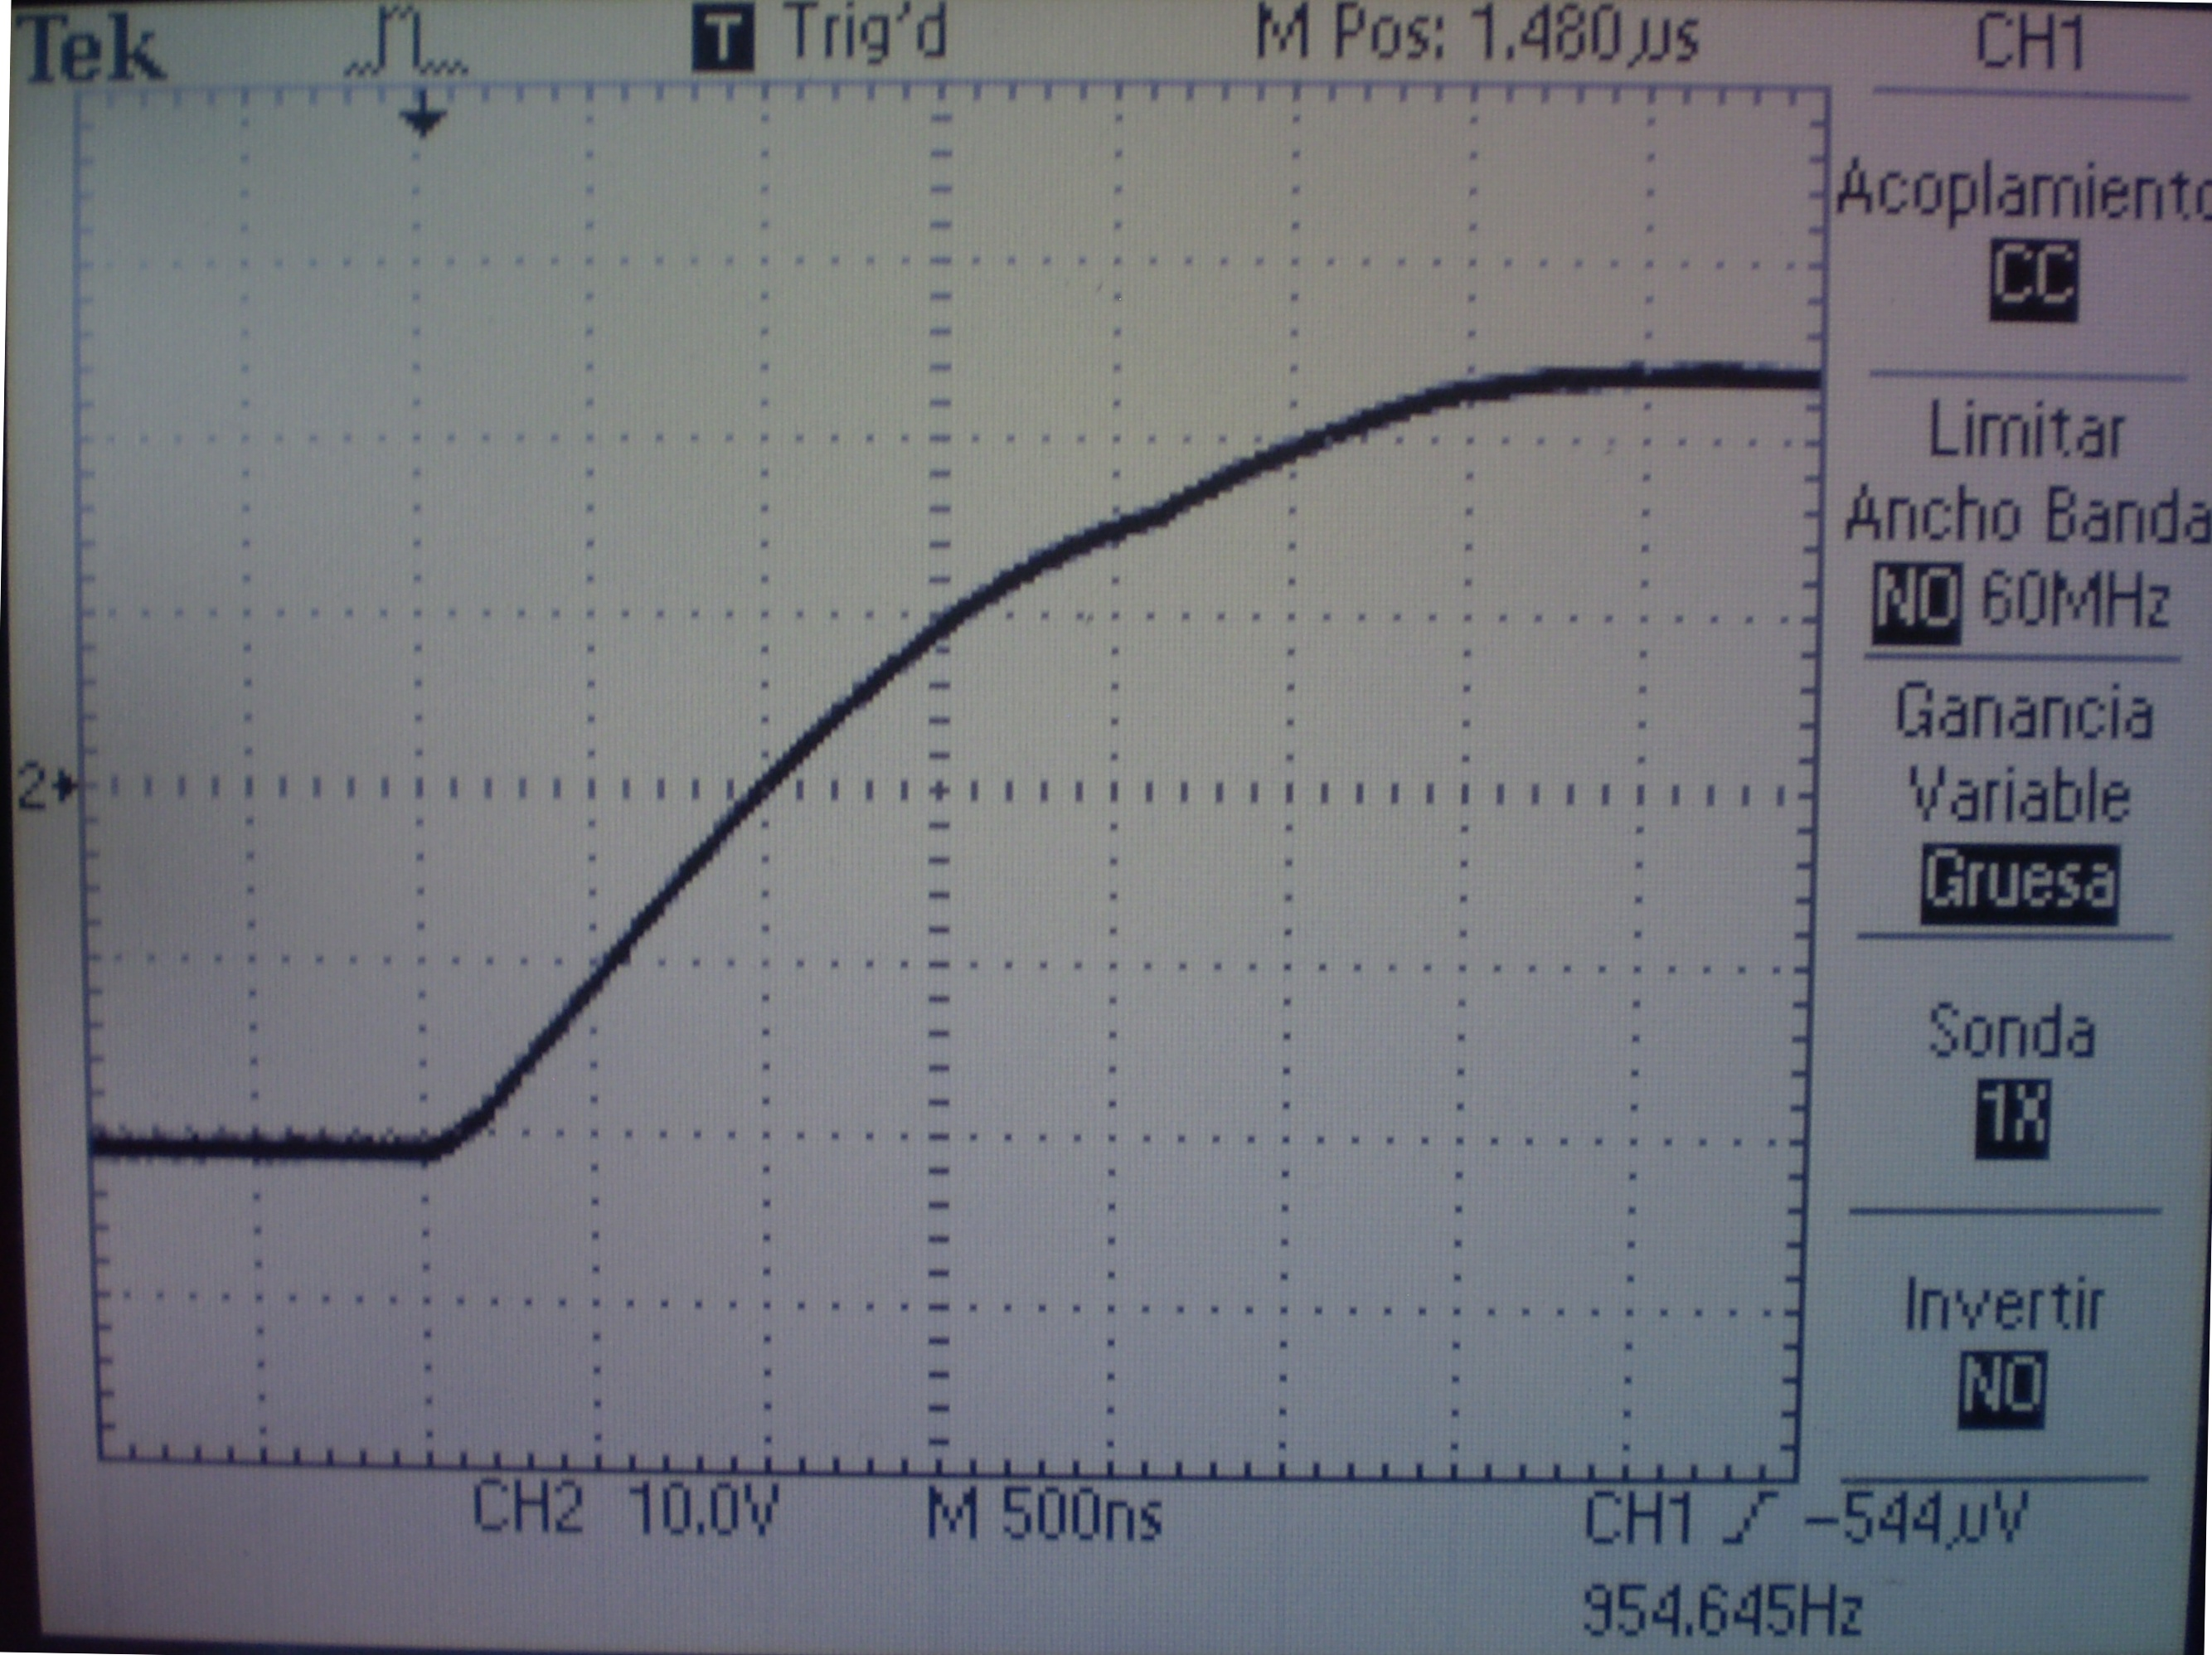
\includegraphics[width=0.9\textwidth]{img/slew_rate_salida.jpg}
\caption{Resultados Slew Rate}
\label{slew_rate_completo} 
\end{figure}


Por lo tanto el Slew Rate se calcula:
$$
Slew Rate =\frac{10V \times 4.4}{6 \times 500ns} = 14.67 \frac{V}{\usec}
$$
\medskip
\subsubsection{Factor de amortiguamiento}

Habiendo medido previamente la impedancia de salida, se calcular el factor de amortiguamiento
como: 
$$
FA = \frac{R_{CARGA NOMINAL}}{Z_{SALIDA}} = 114,28
$$
El factor de amortiguamiento será diferente a distintas frecuencias, el que aqui se calcula es el de 1kHz, debido a que a esa frecuencia se midió la impedancia de salida.

\subsubsection{Distorsión}

Para medir distorsión se utilizó el software Spectralab en conjunto con una placa externa de sonido de baja distorsión, alrededor del $0.003%$, tanto como para regular la amplitud de la señal de entrada como para recibir la señal de salida y poder analizarla en la computadora.
Dado que la placa de sonido contaba con una entrada máxima de $1V_{rms}$, no podría tomar directamente la señal de salida, por lo cual se construyeron dos divisores de tensión. El primero fue para tratar la salida de la señal de $0.3V$, es decir, $V_o=23\times 0.3V=6.9V$. Se utilizaron resistores de AQUI! para atenuar TANTAS! veces y obtener VOLTAJE! a la salida. Idénticamente con la señal de $1V$, se atenuó de $V_o=23\times1V=23V$ a $lalalaV$ con un divisor formado por PEPEPEP!.
De esta forma se fueron realizando las mediciones de distorsión armónica y distorsión por intermodulación, a distintas frecuencias y amplitudes, las cuales se detallaran a continuación.

\subsubsection*{THD}

Para medir THD se generó una onda senoidal de frecuencia $1kHz$ y $7kHz$ de baja tensión, $0.3V_{rms}$ y de alta tensión, $1V_{rms}$. D

\subsubsection*{IMD}